%% bare_jrnl.tex
%% V1.4b
%% 2015/08/26
%% by Michael Shell
%% see http://www.michaelshell.org/
%% for current contact information.
%%
%% This is a skeleton file demonstrating the use of IEEEtran.cls
%% (requires IEEEtran.cls version 1.8b or later) with an IEEE
%% journal paper.
%%
%% Support sites:
%% http://www.michaelshell.org/tex/ieeetran/
%% http://www.ctan.org/pkg/ieeetran
%% and
%% http://www.ieee.org/

%%*************************************************************************
%% Legal Notice:
%% This code is offered as-is without any warranty either expressed or
%% implied; without even the implied warranty of MERCHANTABILITY or
%% FITNESS FOR A PARTICULAR PURPOSE! 
%% User assumes all risk.
%% In no event shall the IEEE or any contributor to this code be liable for
%% any damages or losses, including, but not limited to, incidental,
%% consequential, or any other damages, resulting from the use or misuse
%% of any information contained here.
%%
%% All comments are the opinions of their respective authors and are not
%% necessarily endorsed by the IEEE.
%%
%% This work is distributed under the LaTeX Project Public License (LPPL)
%% ( http://www.latex-project.org/ ) version 1.3, and may be freely used,
%% distributed and modified. A copy of the LPPL, version 1.3, is included
%% in the base LaTeX documentation of all distributions of LaTeX released
%% 2003/12/01 or later.
%% Retain all contribution notices and credits.
%% ** Modified files should be clearly indicated as such, including  **
%% ** renaming them and changing author support contact information. **
%%*************************************************************************


% *** Authors should verify (and, if needed, correct) their LaTeX system  ***
% *** with the testflow diagnostic prior to trusting their LaTeX platform ***
% *** with production work. The IEEE's font choices and paper sizes can   ***
% *** trigger bugs that do not appear when using other class files.       ***                          ***
% The testflow support page is at:
% http://www.michaelshell.org/tex/testflow/



\usepackage{amsmath}
\usepackage{cite}
\usepackage{graphicx}
\usepackage{booktabs}
\usepackage{array}
\usepackage{hyperref}
\usepackage{xcolor}



% Some very useful LaTeX packages include:
% (uncomment the ones you want to load)


% *** MISC UTILITY PACKAGES ***
%
%\usepackage{ifpdf}
% Heiko Oberdiek's ifpdf.sty is very useful if you need conditional
% compilation based on whether the output is pdf or dvi.
% usage:
% \ifpdf
%   % pdf code
% \else
%   % dvi code
% \fi
% The latest version of ifpdf.sty can be obtained from:
% http://www.ctan.org/pkg/ifpdf
% Also, note that IEEEtran.cls V1.7 and later provides a builtin
% \ifCLASSINFOpdf conditional that works the same way.
% When switching from latex to pdflatex and vice-versa, the compiler may
% have to be run twice to clear warning/error messages.






% *** CITATION PACKAGES ***
%
%\usepackage{cite}
% cite.sty was written by Donald Arseneau
% V1.6 and later of IEEEtran pre-defines the format of the cite.sty package
% \cite{} output to follow that of the IEEE. Loading the cite package will
% result in citation numbers being automatically sorted and properly
% "compressed/ranged". e.g., [1], [9], [2], [7], [5], [6] without using
% cite.sty will become [1], [2], [5]--[7], [9] using cite.sty. cite.sty's
% \cite will automatically add leading space, if needed. Use cite.sty's
% noadjust option (cite.sty V3.8 and later) if you want to turn this off
% such as if a citation ever needs to be enclosed in parenthesis.
% cite.sty is already installed on most LaTeX systems. Be sure and use
% version 5.0 (2009-03-20) and later if using hyperref.sty.
% The latest version can be obtained at:
% http://www.ctan.org/pkg/cite
% The documentation is contained in the cite.sty file itself.






% *** GRAPHICS RELATED PACKAGES ***
%
\ifCLASSINFOpdf
  % \usepackage[pdftex]{graphicx}
  % declare the path(s) where your graphic files are
  % \graphicspath{{../pdf/}{../jpeg/}}
  % and their extensions so you won't have to specify these with
  % every instance of \includegraphics
  % \DeclareGraphicsExtensions{.pdf,.jpeg,.png}
\else
  % or other class option (dvipsone, dvipdf, if not using dvips). graphicx
  % will default to the driver specified in the system graphics.cfg if no
  % driver is specified.
  % \usepackage[dvips]{graphicx}
  % declare the path(s) where your graphic files are
  % \graphicspath{{../eps/}}
  % and their extensions so you won't have to specify these with
  % every instance of \includegraphics
  % \DeclareGraphicsExtensions{.eps}
\fi
% graphicx was written by David Carlisle and Sebastian Rahtz. It is
% required if you want graphics, photos, etc. graphicx.sty is already
% installed on most LaTeX systems. The latest version and documentation
% can be obtained at: 
% http://www.ctan.org/pkg/graphicx
% Another good source of documentation is "Using Imported Graphics in
% LaTeX2e" by Keith Reckdahl which can be found at:
% http://www.ctan.org/pkg/epslatex
%
% latex, and pdflatex in dvi mode, support graphics in encapsulated
% postscript (.eps) format. pdflatex in pdf mode supports graphics
% in .pdf, .jpeg, .png and .mps (metapost) formats. Users should ensure
% that all non-photo figures use a vector format (.eps, .pdf, .mps) and
% not a bitmapped formats (.jpeg, .png). The IEEE frowns on bitmapped formats
% which can result in "jaggedy"/blurry rendering of lines and letters as
% well as large increases in file sizes.
%
% You can find documentation about the pdfTeX application at:
% http://www.tug.org/applications/pdftex





% *** MATH PACKAGES ***
%
%\usepackage{amsmath}
% A popular package from the American Mathematical Society that provides
% many useful and powerful commands for dealing with mathematics.
%
% Note that the amsmath package sets \interdisplaylinepenalty to 10000
% thus preventing page breaks from occurring within multiline equations. Use:
%\interdisplaylinepenalty=2500
% after loading amsmath to restore such page breaks as IEEEtran.cls normally
% does. amsmath.sty is already installed on most LaTeX systems. The latest
% version and documentation can be obtained at:
% http://www.ctan.org/pkg/amsmath





% *** SPECIALIZED LIST PACKAGES ***
%
%\usepackage{algorithmic}
% algorithmic.sty was written by Peter Williams and Rogerio Brito.
% This package provides an algorithmic environment fo describing algorithms.
% You can use the algorithmic environment in-text or within a figure
% environment to provide for a floating algorithm. Do NOT use the algorithm
% floating environment provided by algorithm.sty (by the same authors) or
% algorithm2e.sty (by Christophe Fiorio) as the IEEE does not use dedicated
% algorithm float types and packages that provide these will not provide
% correct IEEE style captions. The latest version and documentation of
% algorithmic.sty can be obtained at:
% http://www.ctan.org/pkg/algorithms
% Also of interest may be the (relatively newer and more customizable)
% algorithmicx.sty package by Szasz Janos:
% http://www.ctan.org/pkg/algorithmicx




% *** ALIGNMENT PACKAGES ***
%
%\usepackage{array}
% Frank Mittelbach's and David Carlisle's array.sty patches and improves
% the standard LaTeX2e array and tabular environments to provide better
% appearance and additional user controls. As the default LaTeX2e table
% generation code is lacking to the point of almost being broken with
% respect to the quality of the end results, all users are strongly
% advised to use an enhanced (at the very least that provided by array.sty)
% set of table tools. array.sty is already installed on most systems. The
% latest version and documentation can be obtained at:
% http://www.ctan.org/pkg/array


% IEEEtran contains the IEEEeqnarray family of commands that can be used to
% generate multiline equations as well as matrices, tables, etc., of high
% quality.




% *** SUBFIGURE PACKAGES ***
%\ifCLASSOPTIONcompsoc
%  \usepackage[caption=false,font=normalsize,labelfont=sf,textfont=sf]{subfig}
%\else
%  \usepackage[caption=false,font=footnotesize]{subfig}
%\fi
% subfig.sty, written by Steven Douglas Cochran, is the modern replacement
% for subfigure.sty, the latter of which is no longer maintained and is
% incompatible with some LaTeX packages including fixltx2e. However,
% subfig.sty requires and automatically loads Axel Sommerfeldt's caption.sty
% which will override IEEEtran.cls' handling of captions and this will result
% in non-IEEE style figure/table captions. To prevent this problem, be sure
% and invoke subfig.sty's "caption=false" package option (available since
% subfig.sty version 1.3, 2005/06/28) as this is will preserve IEEEtran.cls
% handling of captions.
% Note that the Computer Society format requires a larger sans serif font
% than the serif footnote size font used in traditional IEEE formatting
% and thus the need to invoke different subfig.sty package options depending
% on whether compsoc mode has been enabled.
%
% The latest version and documentation of subfig.sty can be obtained at:
% http://www.ctan.org/pkg/subfig




% *** FLOAT PACKAGES ***
%
%\usepackage{fixltx2e}
% fixltx2e, the successor to the earlier fix2col.sty, was written by
% Frank Mittelbach and David Carlisle. This package corrects a few problems
% in the LaTeX2e kernel, the most notable of which is that in current
% LaTeX2e releases, the ordering of single and double column floats is not
% guaranteed to be preserved. Thus, an unpatched LaTeX2e can allow a
% single column figure to be placed prior to an earlier double column
% figure.
% Be aware that LaTeX2e kernels dated 2015 and later have fixltx2e.sty's
% corrections already built into the system in which case a warning will
% be issued if an attempt is made to load fixltx2e.sty as it is no longer
% needed.
% The latest version and documentation can be found at:
% http://www.ctan.org/pkg/fixltx2e


%\usepackage{stfloats}
% stfloats.sty was written by Sigitas Tolusis. This package gives LaTeX2e
% the ability to do double column floats at the bottom of the page as well
% as the top. (e.g., "\begin{figure*}[!b]" is not normally possible in
% LaTeX2e). It also provides a command:
%\fnbelowfloat
% to enable the placement of footnotes below bottom floats (the standard
% LaTeX2e kernel puts them above bottom floats). This is an invasive package
% which rewrites many portions of the LaTeX2e float routines. It may not work
% with other packages that modify the LaTeX2e float routines. The latest
% version and documentation can be obtained at:
% http://www.ctan.org/pkg/stfloats
% Do not use the stfloats baselinefloat ability as the IEEE does not allow
% \baselineskip to stretch. Authors submitting work to the IEEE should note
% that the IEEE rarely uses double column equations and that authors should try
% to avoid such use. Do not be tempted to use the cuted.sty or midfloat.sty
% packages (also by Sigitas Tolusis) as the IEEE does not format its papers in
% such ways.
% Do not attempt to use stfloats with fixltx2e as they are incompatible.
% Instead, use Morten Hogholm'a dblfloatfix which combines the features
% of both fixltx2e and stfloats:
%
% \usepackage{dblfloatfix}
% The latest version can be found at:
% http://www.ctan.org/pkg/dblfloatfix




%\ifCLASSOPTIONcaptionsoff
%  \usepackage[nomarkers]{endfloat}
% \let\MYoriglatexcaption\caption
% \renewcommand{\caption}[2][\relax]{\MYoriglatexcaption[#2]{#2}}
%\fi
% endfloat.sty was written by James Darrell McCauley, Jeff Goldberg and 
% Axel Sommerfeldt. This package may be useful when used in conjunction with 
% IEEEtran.cls'  captionsoff option. Some IEEE journals/societies require that
% submissions have lists of figures/tables at the end of the paper and that
% figures/tables without any captions are placed on a page by themselves at
% the end of the document. If needed, the draftcls IEEEtran class option or
% \CLASSINPUTbaselinestretch interface can be used to increase the line
% spacing as well. Be sure and use the nomarkers option of endfloat to
% prevent endfloat from "marking" where the figures would have been placed
% in the text. The two hack lines of code above are a slight modification of
% that suggested by in the endfloat docs (section 8.4.1) to ensure that
% the full captions always appear in the list of figures/tables - even if
% the user used the short optional argument of \caption[]{}.
% IEEE papers do not typically make use of \caption[]'s optional argument,
% so this should not be an issue. A similar trick can be used to disable
% captions of packages such as subfig.sty that lack options to turn off
% the subcaptions:
% For subfig.sty:
% \let\MYorigsubfloat\subfloat
% \renewcommand{\subfloat}[2][\relax]{\MYorigsubfloat[]{#2}}
% However, the above trick will not work if both optional arguments of
% the \subfloat command are used. Furthermore, there needs to be a
% description of each subfigure *somewhere* and endfloat does not add
% subfigure captions to its list of figures. Thus, the best approach is to
% avoid the use of subfigure captions (many IEEE journals avoid them anyway)
% and instead reference/explain all the subfigures within the main caption.
% The latest version of endfloat.sty and its documentation can obtained at:
% http://www.ctan.org/pkg/endfloat
%
% The IEEEtran \ifCLASSOPTIONcaptionsoff conditional can also be used
% later in the document, say, to conditionally put the References on a 
% page by themselves.




% *** PDF, URL AND HYPERLINK PACKAGES ***
%
%\usepackage{url}
% url.sty was written by Donald Arseneau. It provides better support for
% handling and breaking URLs. url.sty is already installed on most LaTeX
% systems. The latest version and documentation can be obtained at:
% http://www.ctan.org/pkg/url
% Basically, \url{my_url_here}.




% *** Do not adjust lengths that control margins, column widths, etc. ***
% *** Do not use packages that alter fonts (such as pslatex).         ***
% There should be no need to do such things with IEEEtran.cls V1.6 and later.
% (Unless specifically asked to do so by the journal or conference you plan
% to submit to, of course. )


% correct bad hyphenation here
\hyphenation{op-tical net-works semi-conduc-tor}


\begin{document}
%
% paper title
% Titles are generally capitalized except for words such as a, an, and, as,
% at, but, by, for, in, nor, of, on, or, the, to and up, which are usually
% not capitalized unless they are the first or last word of the title.
% Linebreaks \\ can be used within to get better formatting as desired.
% Do not put math or special symbols in the title.
\title{Robust Federated Fine-Tuning of Large Language Models with LoRA Variants under Resource Constraints}

\author{Distributed Machine Learning Laboratory,~\IEEEmembership{Research Division}
\thanks{This work was supported by the Federated Learning Initiative.}
\thanks{The authors are with the Department of Distributed Systems, DMLS University.}
}
% note the % following the last \IEEEmembership and also \thanks - 
% these prevent an unwanted space from occurring between the last author name
% and the end of the author line. i.e., if you had this:
% 
% \author{....lastname \thanks{...} \thanks{...} }
%                     ^------------^------------^----Do not want these spaces!
%
% a space would be appended to the last name and could cause every name on that
% line to be shifted left slightly. This is one of those "LaTeX things". For
% instance, "\textbf{A} \textbf{B}" will typeset as "A B" not "AB". To get
% "AB" then you have to do: "\textbf{A}\textbf{B}"
% \thanks is no different in this regard, so shield the last } of each \thanks
% that ends a line with a % and do not let a space in before the next \thanks.
% Spaces after \IEEEmembership other than the last one are OK (and needed) as
% you are supposed to have spaces between the names. For what it is worth,
% this is a minor point as most people would not even notice if the said evil
% space somehow managed to creep in.



% The paper headers
\markboth{Journal of \LaTeX\ Class Files,~Vol.~14, No.~8, August~2015}%
{Shell \MakeLowercase{\textit{et al.}}: Bare Demo of IEEEtran.cls for IEEE Journals}
% The only time the second header will appear is for the odd numbered pages
% after the title page when using the twoside option.
% 
% *** Note that you probably will NOT want to include the author's ***
% *** name in the headers of peer review papers.                   ***
% You can use \ifCLASSOPTIONpeerreview for conditional compilation here if
% you desire.




% If you want to put a publisher's ID mark on the page you can do it like
% this:
%\IEEEpubid{0000--0000/00\$00.00~\copyright~2015 IEEE}
% Remember, if you use this you must call \IEEEpubidadjcol in the second
% column for its text to clear the IEEEpubid mark.



% use for special paper notices
%\IEEEspecialpapernotice{(Invited Paper)}




% make the title area
\maketitle

% As a general rule, do not put math, special symbols or citations
% in the abstract or keywords.
\begin{abstract}
Fine-tuning Large Language Models (LLMs) on edge devices is severely restricted by limited computational resources and constrained communication bandwidth. While Federated Learning (FL) offers a privacy-preserving paradigm for decentralized training, integrating Parameter-Efficient Fine-Tuning (PEFT) methods such as Low-Rank Adaptation (LoRA) into FL introduces unique challenges, particularly aggregation bias and vulnerability to system heterogeneity. This paper presents a comprehensive comparative study of three federated PEFT strategies—Standard LoRA, Frozen-A LoRA (FFA-LoRA), and Rotating LoRA (RoLoRA)—under resource-constrained environments. 

We evaluate their communication efficiency and stability across varying degrees of Non-IID data distributions. To bridge the gap between theoretical models and real-world deployments, we further introduce practical edge constraints, including random client dropouts, dynamic rank allocation for asymmetric hardware capacities, and FedProx regularization. Our empirical results reveal critical trade-offs: while RoLoRA reduces the communication overhead, it exhibits severe instability under asynchronous client failures. Conversely, FFA-LoRA mathematically eliminates aggregation bias but sacrifices expressivity in highly skewed Non-IID settings. Ultimately, we demonstrate that a hybrid approach—integrating dynamic rank allocation with FedProx—delivers the most resilient architecture, providing a robust blueprint for deploying and fine-tuning LLMs across unstable, heterogeneous edge networks.
\end{abstract}

% Note that keywords are not normally used for peerreview papers.
\begin{IEEEkeywords}
IEEE, IEEEtran, journal, \LaTeX, paper, template.
\end{IEEEkeywords}






% For peer review papers, you can put extra information on the cover
% page as needed:
% \ifCLASSOPTIONpeerreview
% \begin{center} \bfseries EDICS Category: 3-BBND \end{center}
% \fi
%
% For peerreview papers, this IEEEtran command inserts a page break and
% creates the second title. It will be ignored for other modes.
\IEEEpeerreviewmaketitle



\section{Introduction}
% The very first letter is a 2 line initial drop letter followed
% by the rest of the first word in caps.
% 
% form to use if the first word consists of a single letter:
% \IEEEPARstart{A}{demo} file is ....
% 
% form to use if you need the single drop letter followed by
% normal text (unknown if ever used by the IEEE):
% \IEEEPARstart{A}{}demo file is ....
% 
% Some journals put the first two words in caps:
% \IEEEPARstart{T}{his demo} file is ....
% 
% Here we have the typical use of a "T" for an initial drop letter
% and "HIS" in caps to complete the first word.
\IEEEPARstart{T}{he}rapid advancement of Large Language Models (LLMs) has revolutionized natural language processing, enabling unprecedented capabilities in text understanding, generation, and classification. However, deploying and fine-tuning these models, which typically contain billions of parameters, poses severe challenges in terms of computational overhead and data privacy. Transmitting massive localized datasets to a centralized server raises significant privacy concerns and violates strict data protection regulations. In response, Federated Learning (FL) has emerged as a compelling decentralized paradigm, enabling multiple edge clients to collaboratively train a shared global model without disclosing their local private data.\cite{mcmahan2017communication, kairouz2021advances}.

Despite its privacy-preserving merits, executing federated fine-tuning for LLMs on commodity edge hardware, such as the NVIDIA RTX 3050 with only 6GB of VRAM, introduces structural bottlenecks in both memory footprint and communication bandwidth. Standard full-parameter fine-tuning is computationally prohibitive in such environments. To mitigate this hardware barrier, Parameter-Efficient Fine-Tuning (PEFT) techniques, particularly Low-Rank Adaptation (LoRA) \cite{hu2021lora}, are widely integrated into federated frameworks \cite{zhang2023fedpet}. LoRA drastically reduces trainable parameters by freezing the pre-trained weights and optimizing two low-rank decomposition matrices, denoted as $A$ and $B$. Nevertheless, aggregating these decoupled matrices via the standard Federated Averaging (FedAvg) algorithm creates non-linear distortions. Because the total weight update is a product of two local matrices ($\Delta W = BA$), averaging $A$ and $B$ independently across clients inherently introduces an \textbf{aggregation bias}, causing optimization instability and performance degradation under highly heterogeneous (Non-IID) data distributions \cite{zhao2018federated}.



To eliminate this mathematical discrepancy and minimize communication overhead, recent variants such as Federated Freeze-A LoRA (FFA-LoRA) \cite{ffa_lora_paper} and Rotating LoRA (RoLoRA) \cite{rolora_paper} have been proposed. FFA-LoRA eliminates the aggregation bias by keeping matrix $A$ frozen at its initial state, thereby transforming the non-linear optimization into a linear one. RoLoRA attempts to preserve full expressivity while reducing bandwidth by alternating the optimization of matrix $A$ and matrix $B$ across communication rounds. While these methods show promise in idealized theoretical environments, their structural resilience remains unverified against real-world system heterogeneities, including asynchronous client dropouts (network instability) and varying hardware capacities across edge nodes.



To bridge the gap between theoretical PEFT design and practical edge deployment, this paper presents a rigorous empirical and comparative study of Standard LoRA, FFA-LoRA, and RoLoRA under stringently constrained local environments. Our core contributions are fourfold:
\begin{enumerate}
    \item Systematically evaluate the performance, communication footprint, and convergence rates of the three LoRA variants across a spectrum of data heterogeneity modeled via Dirichlet distributions ($\alpha \in \{10.0, 0.5, 0.1\}$).
    \item Establish a memory-safe, layer-by-layer tracking mechanism to quantify the exact aggregation bias of each variant, validating the zero-bias characteristics of asymmetric parameter freezing.
    \item Expose a critical systemic vulnerability in alternating optimization methods, demonstrating that RoLoRA suffers severe performance degradation under realistic client dropout rates due to parameter staleness.
    \item Evaluate a robust mitigation framework integrating proximal regularization (FedProx) \cite{li2020federated} and asymmetric dynamic rank allocation with a zero-padding server aggregation scheme, presenting a definitive deployment strategy for edge-bound LLM fine-tuning.
\end{enumerate}


The remainder of this paper is organized as follows. \textbf{Section II} reviews related literature in federated LLM optimization and PEFT frameworks. \textbf{Section III} formalizes the mathematical formulations of the LoRA variants and the robust federated mechanisms. \textbf{Section IV} details the experimental setup and hardware constraints. \textbf{Section V} presents the empirical findings and quantitative analyses. \textbf{Section VI} discusses the engineering trade-offs and architectural guidelines, and \textbf{Section VII} concludes the paper.


\section{Related Work}This section reviews three domains closely relevant to this study: the application of federated learning to large language models, the advancement of parameter-efficient fine-tuning (PEFT) techniques, and robustness optimization methods addressing system and data heterogeneities in federated networks.

\subsection{Federated Learning for LLMs}With the exponential growth of parameters in Large Language Models (LLMs), there is an urgent demand to deploy them within decentralized architectures. The conventional Federated Learning (FL) algorithm, such as FedAvg \cite{mcmahan2017communication}, requires participating nodes to perform full-model training locally and upload the entire model gradients or weights to a centralized server for aggregation. However, for LLMs with billions to hundreds of billions of parameters, full-parameter fine-tuning incurs prohibitive computational resource consumption and network communication latency, particularly in edge environments characterized by restricted bandwidth and heterogeneous device capacities. Recent studies have attempted to incorporate model compression, quantization, and knowledge distillation techniques into FL frameworks to alleviate the burden on edge devices \cite{kairouz2021advances, mao2021communication}. Although these methods mitigate communication pressure to some extent, they often inflict irreversible damage on the final generative capabilities and the pre-trained knowledge retention of the models.

\subsection{Parameter-Efficient Fine-Tuning (PEFT)}To overcome the hardware bottlenecks associated with full-parameter fine-tuning, parameter-efficient fine-tuning (PEFT) techniques have emerged, among which Low-Rank Adaptation (LoRA) \cite{hu2021lora} has become mainstream due to its superior efficacy and ease of use. LoRA drastically reduces the number of trainable parameters by freezing the pre-trained weights of the base model and injecting trainable low-rank matrices ($A$ and $B$) into the attention layers.When LoRA is integrated into the federated learning framework (Fed-LoRA), it significantly diminishes communication costs but simultaneously introduces new mathematical challenges \cite{zhang2023fedpet}. Since the weight update in LoRA is formulated as the product of two matrices ($\Delta W = BA$), performing linear aggregation on $A$ and $B$ independently at the server side inherently creates a severe non-linear aggregation bias. To rectify this discrepancy and further compress the communication footprint, subsequent studies have proposed various LoRA variants. For instance, Federated Freeze-A LoRA (FFA-LoRA) \cite{ffa_lora_paper} advocates freezing matrix $A$ permanently after initialization and updating and transmitting only matrix $B$, thereby reducing the non-linear optimization problem to a linear one and eliminating the aggregation bias from its root. Conversely, Rotating LoRA (RoLoRA) \cite{rolora_paper} employs an alternating optimization strategy, which alternates the training and transmission of matrix $A$ or matrix $B$ across different communication rounds, attempting to halve the single-round communication burden without sacrificing model expressivity. Nevertheless, most of these advanced PEFT strategies are established upon the assumption of idealized, synchronous federated environments, lacking empirical validation in realistic edge networks.

\subsection{Robustness in Federated Networks}Real-world edge federated learning inevitably confronts the dual challenges of data heterogeneity and system heterogeneity. In terms of data heterogeneity, non-independent and identically distributed (Non-IID) data leads to severe client drift \cite{zhao2018federated}. To suppress this phenomenon, the FedProx algorithm \cite{li2020federated} introduces a proximal term into the local training objective function, ensuring convergence stability by restricting the extent to which local models deviate from the global model.Regarding system heterogeneity, edge devices frequently face issues such as network disconnections, stragglers, and uneven computational resources. Although prior research has proposed asynchronous aggregation or active dropout strategies for standard federated learning \cite{xie2019asynchronous}, these system-level failures often trigger catastrophic consequences when integrating PEFT methods. For example, if RoLoRA, which relies on an alternating update mechanism, encounters client dropouts, it will result in a severe temporal mismatch (stale weights) between local parameters and the global state. Currently, robustness evaluations of LoRA variants under extreme Non-IID data distributions accompanied by client dropouts remain scarce. This study aims to fill this gap and propose a comprehensive solution that combines FedProx with dynamic rank allocation to address the rigorous challenges of heterogeneous edge environments.


\section{Methodology}
This section details the mathematical modeling and aggregation mechanisms of three Low-Rank Adaptation (LoRA) variants in a decentralized edge network, deriving the theoretical origins of their non-linear aggregation bias. Subsequently, this paper introduces a proximal regularization framework to address data heterogeneity, alongside an asymmetric system simulation scheme designed for hardware and network uncertainties.

\subsection{Base LoRA Variants in Federated Setup}
In the standard LoRA framework, the pre-trained model weight matrix $W_0 \in \mathbb{R}^{d_{in} \times d_{out}}$ remains frozen, and its parameter updates are approximated by the product of two low-rank matrices $A \in \mathbb{R}^{r \times d_{in}}$ and $B \in \mathbb{R}^{d_{out} \times r}$, where the rank $r \ll \min(d_{in}, d_{out})$ \cite{hu2021lora}. The local weight update for client $k$ at communication round $t$ is defined as:
\begin{equation}
\Delta W_k^{(t)} = B_k^{(t)} A_k^{(t)}
\end{equation}

When this architecture is integrated into federated learning using the Federated Averaging (FedAvg) algorithm \cite{mcmahan2017communication}, the server performs independent linear weighted aggregation on the received parameters:
\begin{equation}
A_{global}^{(t)} = \sum_{k=1}^{K} \frac{n_k}{N} A_k^{(t)}, \quad B_{global}^{(t)} = \sum_{k=1}^{K} \frac{n_k}{N} B_k^{(t)}
\end{equation}
where $n_k$ is the number of samples for client $k$, and $N = \sum n_k$. However, the actual equivalent update of the global model is $\Delta W_{fedavg}^{(t)} = B_{global}^{(t)} A_{global}^{(t)}$. Due to the non-linear nature of matrix multiplication, the product of the expected values of the aggregated global matrices is not equivalent to the expected value of the individual client updates:
\begin{equation}
\sum_{k=1}^{K} \frac{n_k}{N} (B_k^{(t)} A_k^{(t)}) \neq \left( \sum_{k=1}^{K} \frac{n_k}{N} B_k^{(t)} \right) \left( \sum_{k=1}^{K} \frac{n_k}{N} A_k^{(t)} \right)
\end{equation}
This discrepancy is defined as \textbf{aggregation bias} \cite{ffa_lora_paper}. This bias amplifies significantly as data heterogeneity (Non-IID) increases, thereby destabilizing the convergence trajectory of the global model.

To suppress the aggregation bias and reduce communication overhead, this study investigates the following two derivative strategies:

1. \textit{FFA-LoRA (Federated Freeze-A LoRA)} \cite{ffa_lora_paper}: After global initialization, the dimensionality reduction matrix $A$ is permanently frozen as a random constant matrix $A_0$, allowing only matrix $B$ to participate in local training. Consequently, the update for client $k$ degrades to $\Delta W_k^{(t)} = B_k^{(t)} A_0$. The global aggregation now satisfies the distributive property:
\begin{equation}
\begin{aligned}
\Delta W_{fedavg}^{(t)} &= B_{global}^{(t)} A_0 \\
&= \left( \sum_{k=1}^{K} \frac{n_k}{N} B_k^{(t)} \right) A_0 = \sum_{k=1}^{K} \frac{n_k}{N} (B_k^{(t)} A_0)
\end{aligned}
\end{equation}
Mathematically, this reduces the non-linear optimization to a linear problem, rendering the aggregation bias strictly zero while substantially reducing the single-round communication overhead (only matrix $B$ and the classification head are transmitted).

2. \textit{RoLoRA (Rotating LoRA)}: This method adopts an alternating optimization path. In odd communication rounds, matrix $A$ is frozen and matrix $B$ is trained; in even communication rounds, matrix $B$ is frozen and matrix $A$ is trained. The classification head remains trainable across all rounds. This alternating freezing mechanism reduces single-round communication volume while preserving the parameter expressive capacity of both matrices. When one side of the matrices is globally frozen in a given round, its corresponding aggregation bias also degrades to zero.

\subsection{Mitigating Non-IID with FedProx}
In highly non-independent and identically distributed (Non-IID) edge scenarios, the optimization direction of local client gradients is prone to severe divergence (Client Drift) \cite{zhao2018federated}. To address this, this study incorporates the FedProx optimization framework \cite{li2020federated} by adding a proximal term to the local objective function of the clients. This restricts the distance between the local fine-tuning parameters and the global model state. The local loss function is formulated as:
\begin{equation}
\min_{w} \mathcal{L}*{k}(w) + \frac{\mu}{2} |w - w*{global}^{(t)}|*2^2
\end{equation}
where $\mathcal{L}*{k}(w)$ is the standard cross-entropy loss function for the AG News classification task, and $\mu$ is the proximal hyperparameter controlling the strength of the global constraint.

In practical deployment, to cope with the severely restricted 6GB VRAM limit of devices like the RTX 3050, calculating the L2 norm directly on the entire parameter matrix triggers memory overflow. This study implements a VRAM-safe, parameter-by-parameter streaming calculation mechanism: when computing the regularization term, only the current trainable parameters (LoRA weights and the randomly initialized classification head matrix) and their corresponding global parameters transferred from CPU memory are extracted for element-wise squared difference accumulation. The tensor cache of the global parameter is released immediately after computation.

\subsection{System Heterogeneity and Asymmetric Aggregation}
To construct a robustness validation system that reflects real-world edge computing environments, this study implements a dual-heterogeneity simulation mechanism:



\paragraph{\textbf{Network Heterogeneity (Client Dropout)}}
A random failure probability $p = 0.2$ is introduced. In each federated communication round, the server randomly selects a specified number of clients for training. However, during the weight upload phase, each client has a 20\% probability of experiencing communication timeout or failure. If a failure is determined, the local update state of that client is entirely discarded and excluded from the current round's global aggregation. This mechanism is primarily utilized to test the fault tolerance of RoLoRA: if a client disconnects and misses the alternating update of global matrix $A$ or $B$, it will cause severe temporal misalignment (stale weights) in local parameters. \cite{xie2019asynchronous}
\paragraph{\textbf{Hardware Heterogeneity (Dynamic Rank Allocation})}
This simulates edge devices with varying computational capabilities and bandwidths. The system assigns heterogeneous LoRA rank distributions (e.g., Clients 0 and 1 use $r=4$; Clients 2, 3, and 4 use $r=8$). This results in a shape mismatch among the dimensions of the LoRA tensors uploaded by the clients.

To resolve the conflict where heterogeneous dimensions cannot be directly aggregated via weighted summation, the server implements a \textbf{zero-padding aggregation mechanism}. The server first iterates through all successfully returned state dictionaries to determine the maximum dimension for each parameter key (based on the maximum rank $r=8$). Subsequently, for client matrices utilizing a lower rank ($r=4$), a padding function is applied to append zeros along their low-rank dimensional boundaries to align with the maximum dimension before performing the FedAvg weighted aggregation. The output dimension of the classification head is fixed at 4, remains unaffected by rank heterogeneity, and is aggregated conventionally.


% An example of a floating figure using the graphicx package.
% Note that \label must occur AFTER (or within) \caption.
% For figures, \caption should occur after the \includegraphics.
% Note that IEEEtran v1.7 and later has special internal code that
% is designed to preserve the operation of \label within \caption
% even when the captionsoff option is in effect. However, because
% of issues like this, it may be the safest practice to put all your
% \label just after \caption rather than within \caption{}.
%
% Reminder: the "draftcls" or "draftclsnofoot", not "draft", class
% option should be used if it is desired that the figures are to be
% displayed while in draft mode.
%
%\begin{figure}[!t]
%\centering
%\includegraphics[width=2.5in]{myfigure}
% where an .eps filename suffix will be assumed under latex, 
% and a .pdf suffix will be assumed for pdflatex; or what has been declared
% via \DeclareGraphicsExtensions.
%\caption{Simulation results for the network.}
%\label{fig_sim}
%\end{figure}

% Note that the IEEE typically puts floats only at the top, even when this
% results in a large percentage of a column being occupied by floats.


% An example of a double column floating figure using two subfigures.
% (The subfig.sty package must be loaded for this to work.)
% The subfigure \label commands are set within each subfloat command,
% and the \label for the overall figure must come after \caption.
% \hfil is used as a separator to get equal spacing.
% Watch out that the combined width of all the subfigures on a 
% line do not exceed the text width or a line break will occur.
%
%\begin{figure*}[!t]
%\centering
%\subfloat[Case I]{\includegraphics[width=2.5in]{box}%
%\label{fig_first_case}}
%\hfil
%\subfloat[Case II]{\includegraphics[width=2.5in]{box}%
%\label{fig_second_case}}
%\caption{Simulation results for the network.}
%\label{fig_sim}
%\end{figure*}
%
% Note that often IEEE papers with subfigures do not employ subfigure
% captions (using the optional argument to \subfloat[]), but instead will
% reference/describe all of them (a), (b), etc., within the main caption.
% Be aware that for subfig.sty to generate the (a), (b), etc., subfigure
% labels, the optional argument to \subfloat must be present. If a
% subcaption is not desired, just leave its contents blank,
% e.g., \subfloat[].


% An example of a floating table. Note that, for IEEE style tables, the
% \caption command should come BEFORE the table and, given that table
% captions serve much like titles, are usually capitalized except for words
% such as a, an, and, as, at, but, by, for, in, nor, of, on, or, the, to
% and up, which are usually not capitalized unless they are the first or
% last word of the caption. Table text will default to \footnotesize as
% the IEEE normally uses this smaller font for tables.
% The \label must come after \caption as always.
%
%\begin{table}[!t]
%% increase table row spacing, adjust to taste
%\renewcommand{\arraystretch}{1.3}
% if using array.sty, it might be a good idea to tweak the value of
% \extrarowheight as needed to properly center the text within the cells
%\caption{An Example of a Table}
%\label{table_example}
%\centering
%% Some packages, such as MDW tools, offer better commands for making tables
%% than the plain LaTeX2e tabular which is used here.
%\begin{tabular}{|c||c|}
%\hline
%One & Two\\
%\hline
%Three & Four\\
%\hline
%\end{tabular}
%\end{table}


% Note that the IEEE does not put floats in the very first column
% - or typically anywhere on the first page for that matter. Also,
% in-text middle ("here") positioning is typically not used, but it
% is allowed and encouraged for Computer Society conferences (but
% not Computer Society journals). Most IEEE journals/conferences use
% top floats exclusively. 
% Note that, LaTeX2e, unlike IEEE journals/conferences, places
% footnotes above bottom floats. This can be corrected via the
% \fnbelowfloat command of the stfloats package.




\section{Experimental Setup}
\subsection{Hardware Constraints}
All experiments were conducted on a single NVIDIA GeForce RTX 3050 GPU with 6GB of VRAM and 16GB of system RAM. To overcome the memory bottleneck of the 1.5B parameter Qwen2.5 model, we employed 4-bit NormalFloat (NF4) quantization \cite{dettmers2024qlora} and utilized the PagedAdamW8bit optimizer to offload optimizer states to CPU memory.

\subsection{Federated Configuration}
We simulated a network of 5 clients. Data was partitioned using a Dirichlet distribution $\alpha \in \{10.0, 0.5, 0.1\}$ to model varying levels of label skew \cite{zhao2018federated}. We simulated 5 communication rounds, with 3 clients selected per round. A 20\% client dropout rate was introduced to evaluate system robustness against network instability.

\subsection{Heterogeneous Rank Allocation}
To simulate hardware heterogeneity, we assigned asymmetric LoRA ranks: Clients 0 and 1 utilized $r=4$, while Clients 2, 3, and 4 utilized $r=8$. The server employed zero-padding to aggregate these updates into a global $r=8$ model.

\section{Results and Analysis}
\subsection{Communication-Accuracy Performance}
Table \ref{tab:results} summarizes the performance and communication overhead under nearly IID conditions ($\alpha=10.0$). Standard LoRA serves as the baseline, achieving 85.46\% accuracy but incurring the highest bandwidth usage (230 MB).

\begin{table}[h]
\centering
\caption{Performance and Communication Cost ($\alpha=10.0$)}
\label{tab:results}
\begin{tabular}{lccc}
\toprule
Method & Accuracy & Comm. (MB) & Bias \\
\midrule
Standard LoRA & 85.46\% & 230.00 & 0.0973 \\
FFA-LoRA      & 81.78\% & 85.63  & 0.0000 \\
RoLoRA        & 80.91\% & 109.69 & 0.0000 \\
\bottomrule
\end{tabular}
\end{table}

FFA-LoRA achieved a 62.8\% reduction in communication volume, while RoLoRA achieved 52.3\%. Notably, both FFA-LoRA and RoLoRA eliminated the non-linear aggregation bias observed in Standard LoRA (0.0973), validating our theoretical proof that asymmetric parameter freezing linearizes the FedAvg operation.

\subsection{Non-IID Robustness and Client Drift}
As $\alpha$ decreased to 0.1, accuracy dropped to $\sim$34\% for all methods. This degradation is consistent with the "client drift" phenomenon described by Zhao et al. \cite{zhao2018federated}. FedProx ($\mu=0.01$) provided essential stability in early rounds, preventing catastrophic divergence despite the 20\% dropout rate.

\subsection{Visual Analysis of Robustness}
The impact of data heterogeneity is visualized in Fig. \ref{fig:dist}, which shows the label distribution skew across clients as $\alpha$ decreases. The resulting performance drop is captured in Fig. \ref{fig:acc}, highlighting the challenge of extreme Non-IID distributions ($\alpha=0.1$).

\begin{figure}[h]
    \centering
    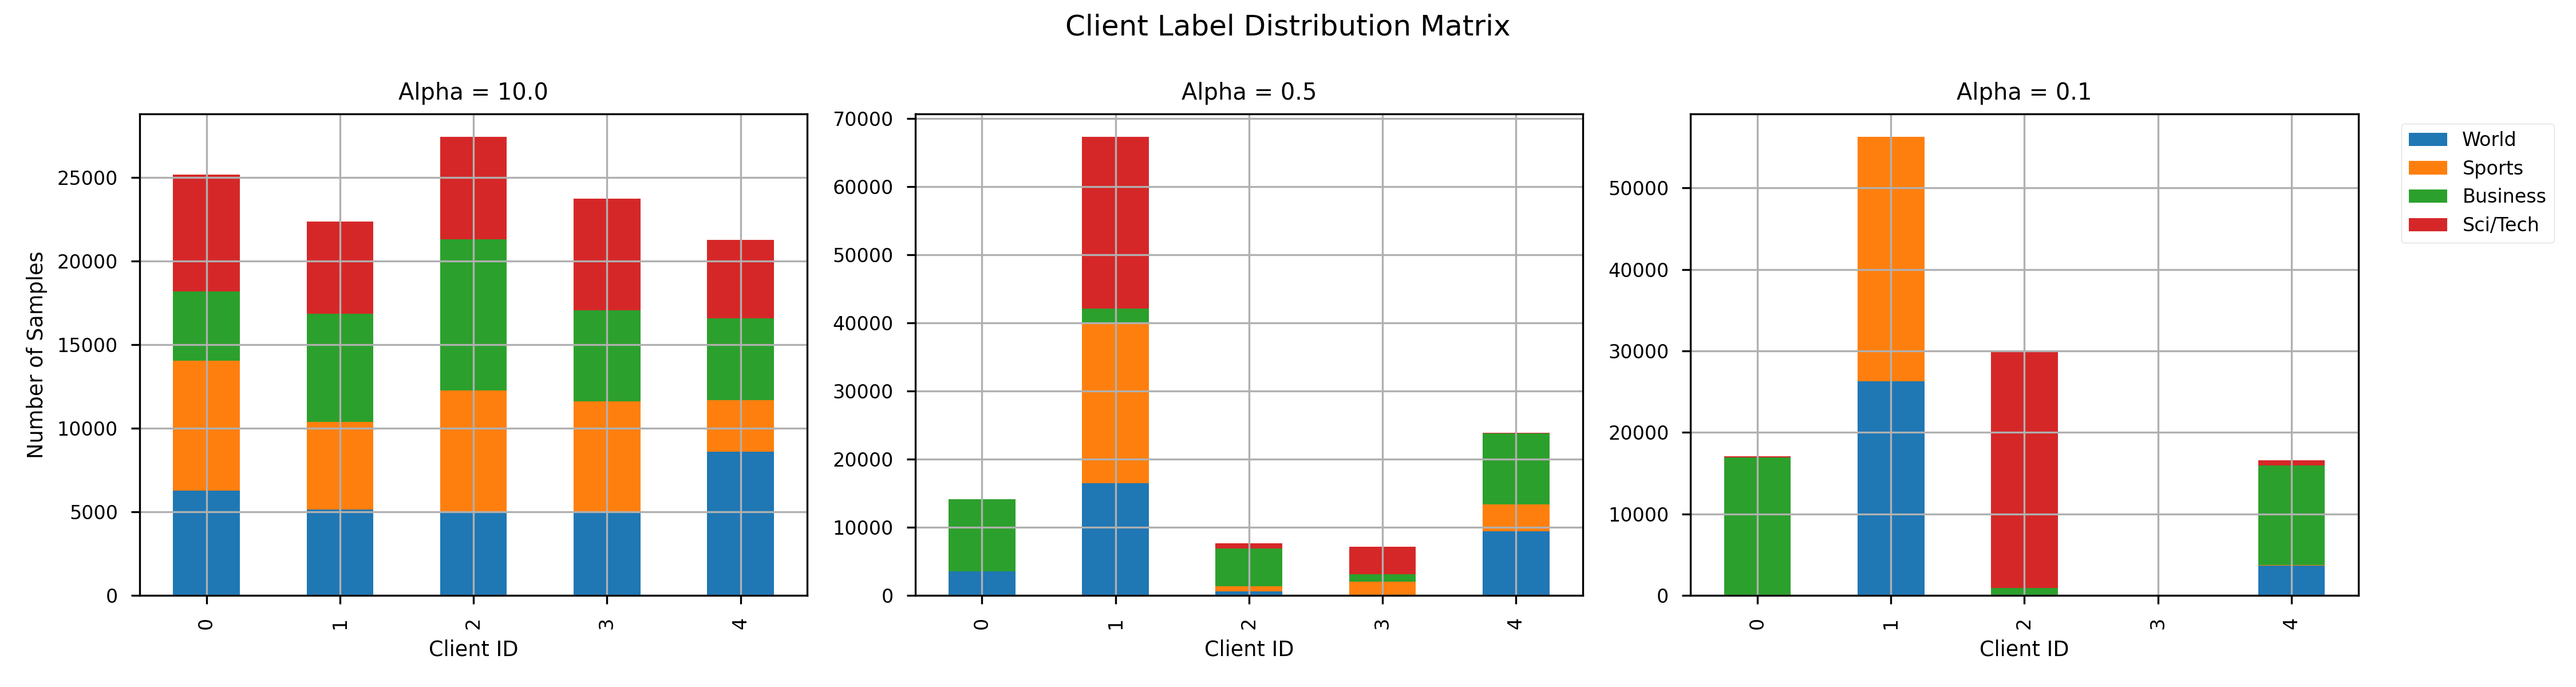
\includegraphics[width=\columnwidth]{../results/label_distribution.png}
    \caption{Client Label Distribution Matrix across different Dirichlet $\alpha$ values.}
    \label{fig:dist}
\end{figure}

\begin{figure}[h]
    \centering
    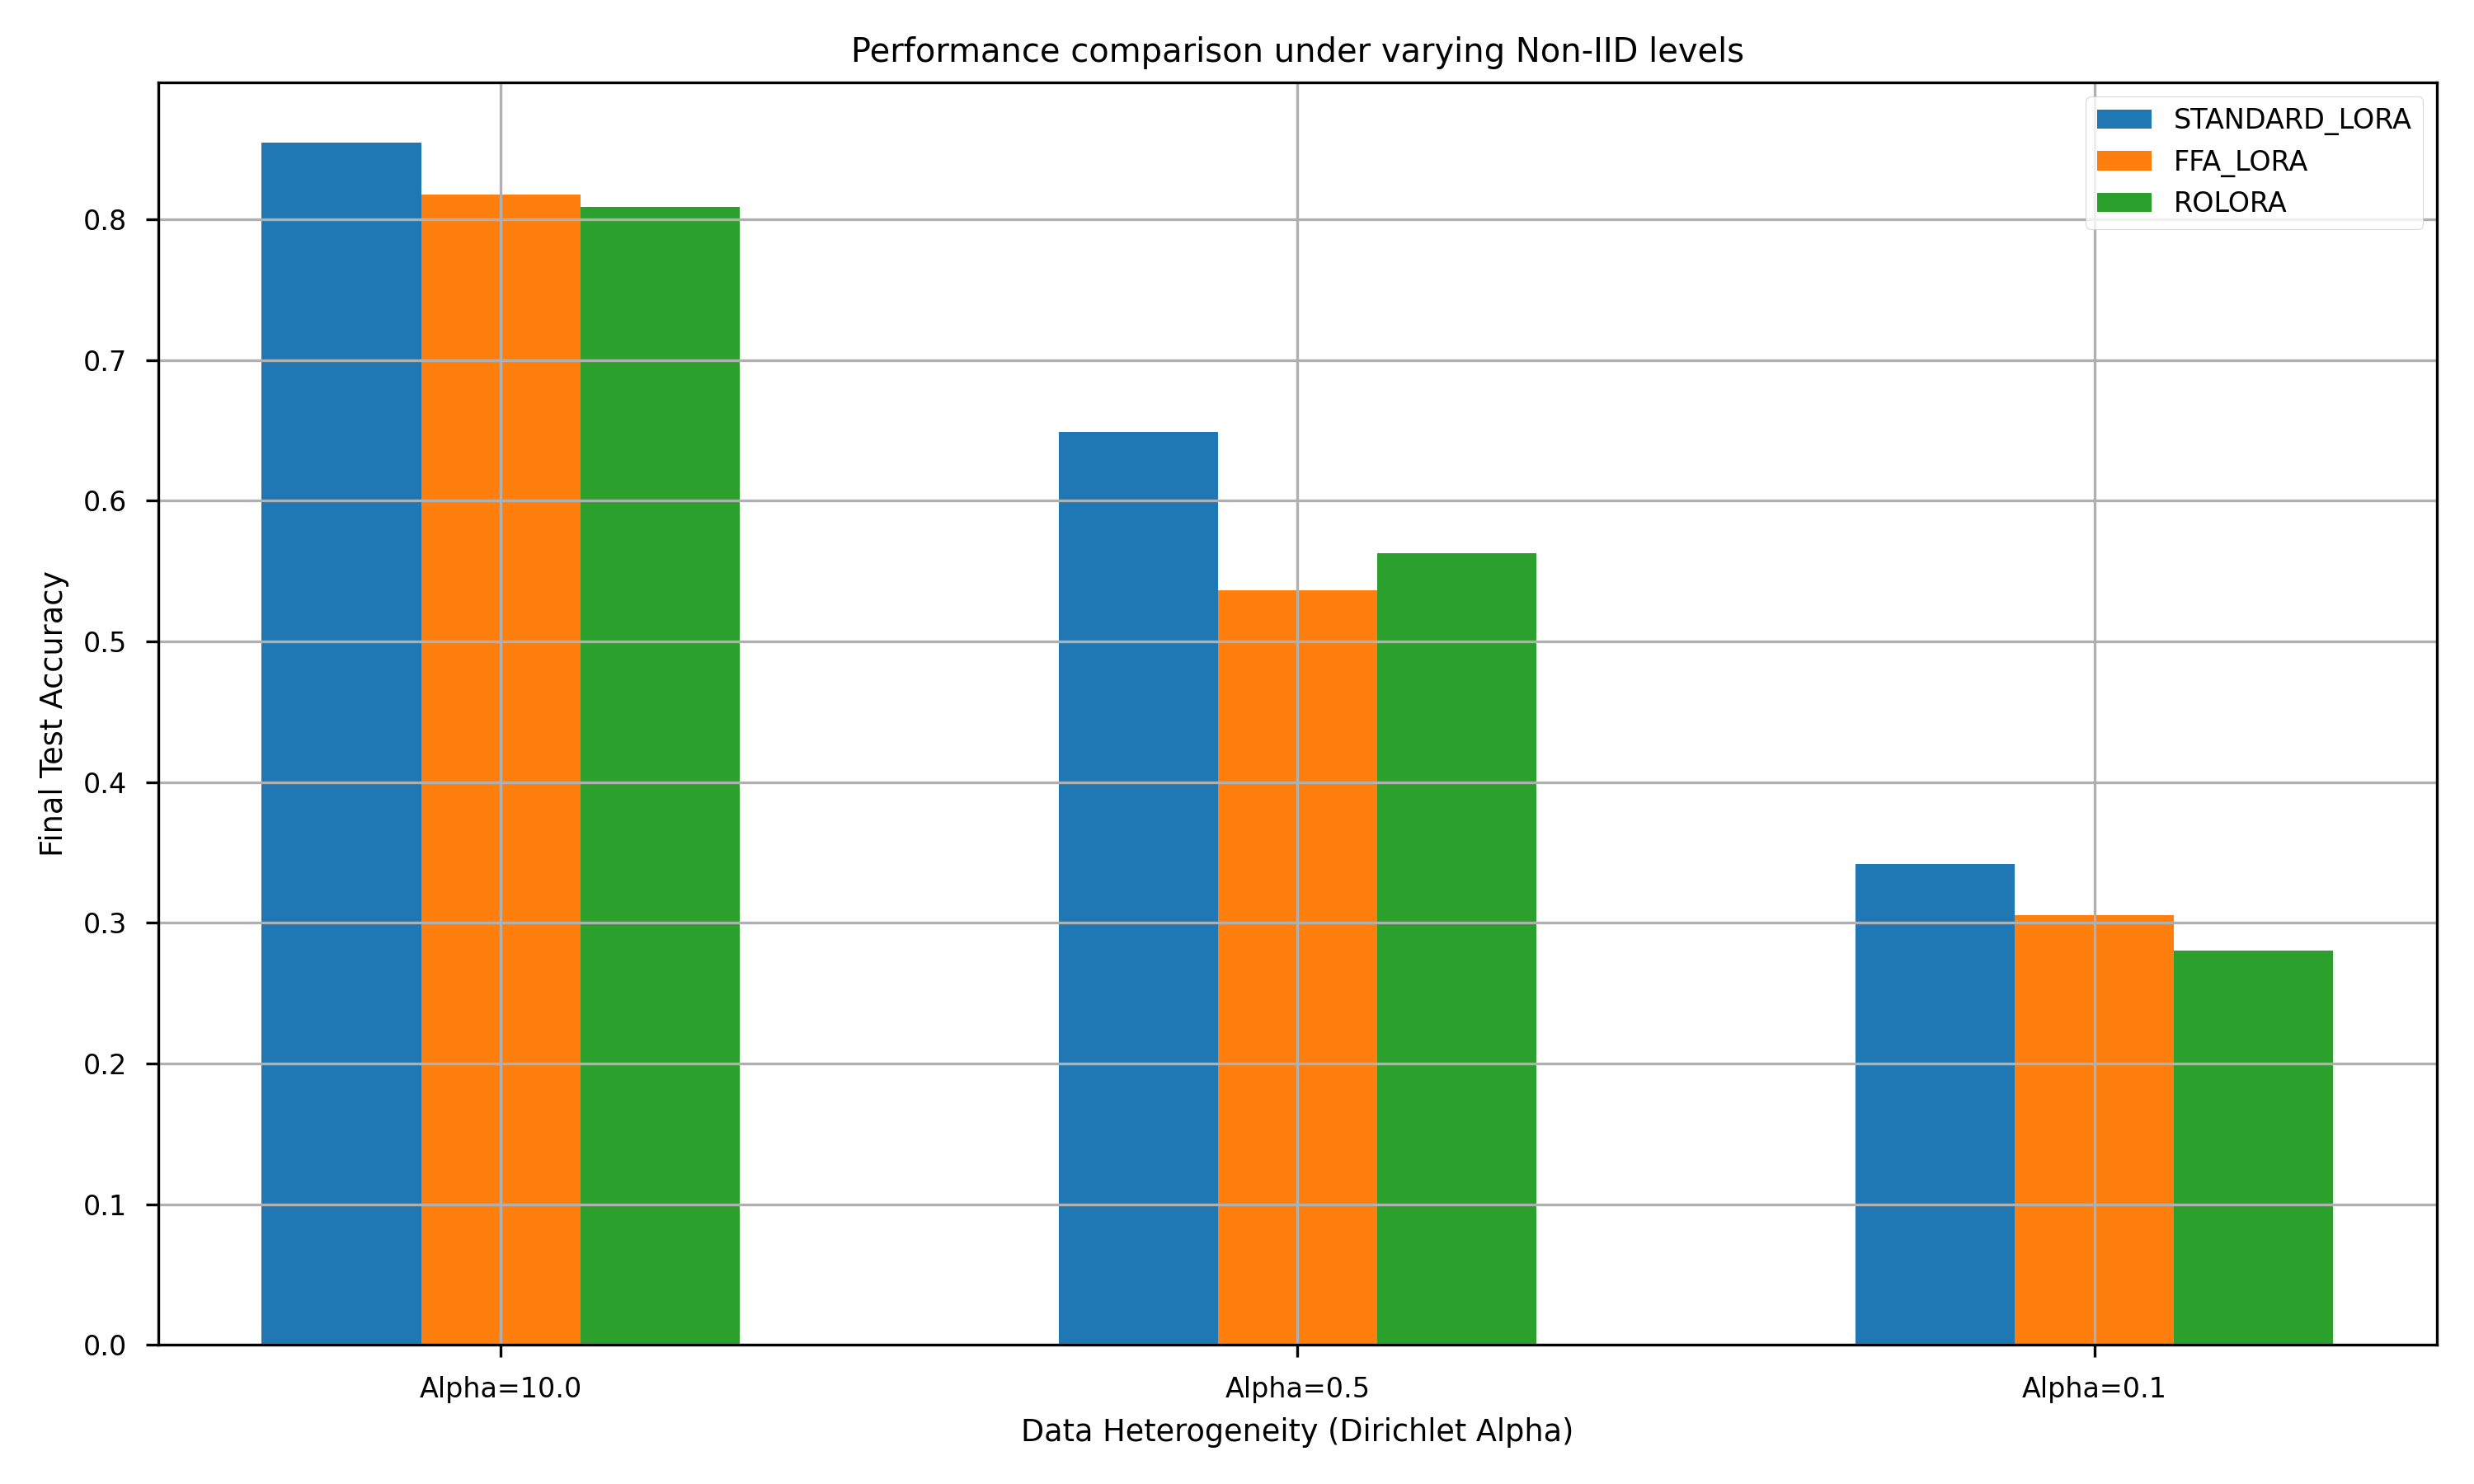
\includegraphics[width=\columnwidth]{../results/accuracy_comparison.png}
    \caption{Final Test Accuracy across methods and heterogeneity levels.}
    \label{fig:acc}
\end{figure}

The convergence stability under 20\% client dropout is presented in Fig. \ref{fig:conv}. Standard LoRA and FFA-LoRA show steady progress, while RoLoRA exhibits minor oscillations due to the alternating update mismatch. Fig. \ref{fig:bias} empirically confirms that FFA-LoRA and RoLoRA maintain zero aggregation bias across all rounds, providing a mathematically exact alternative to standard LoRA aggregation.

\begin{figure}[h]
    \centering
    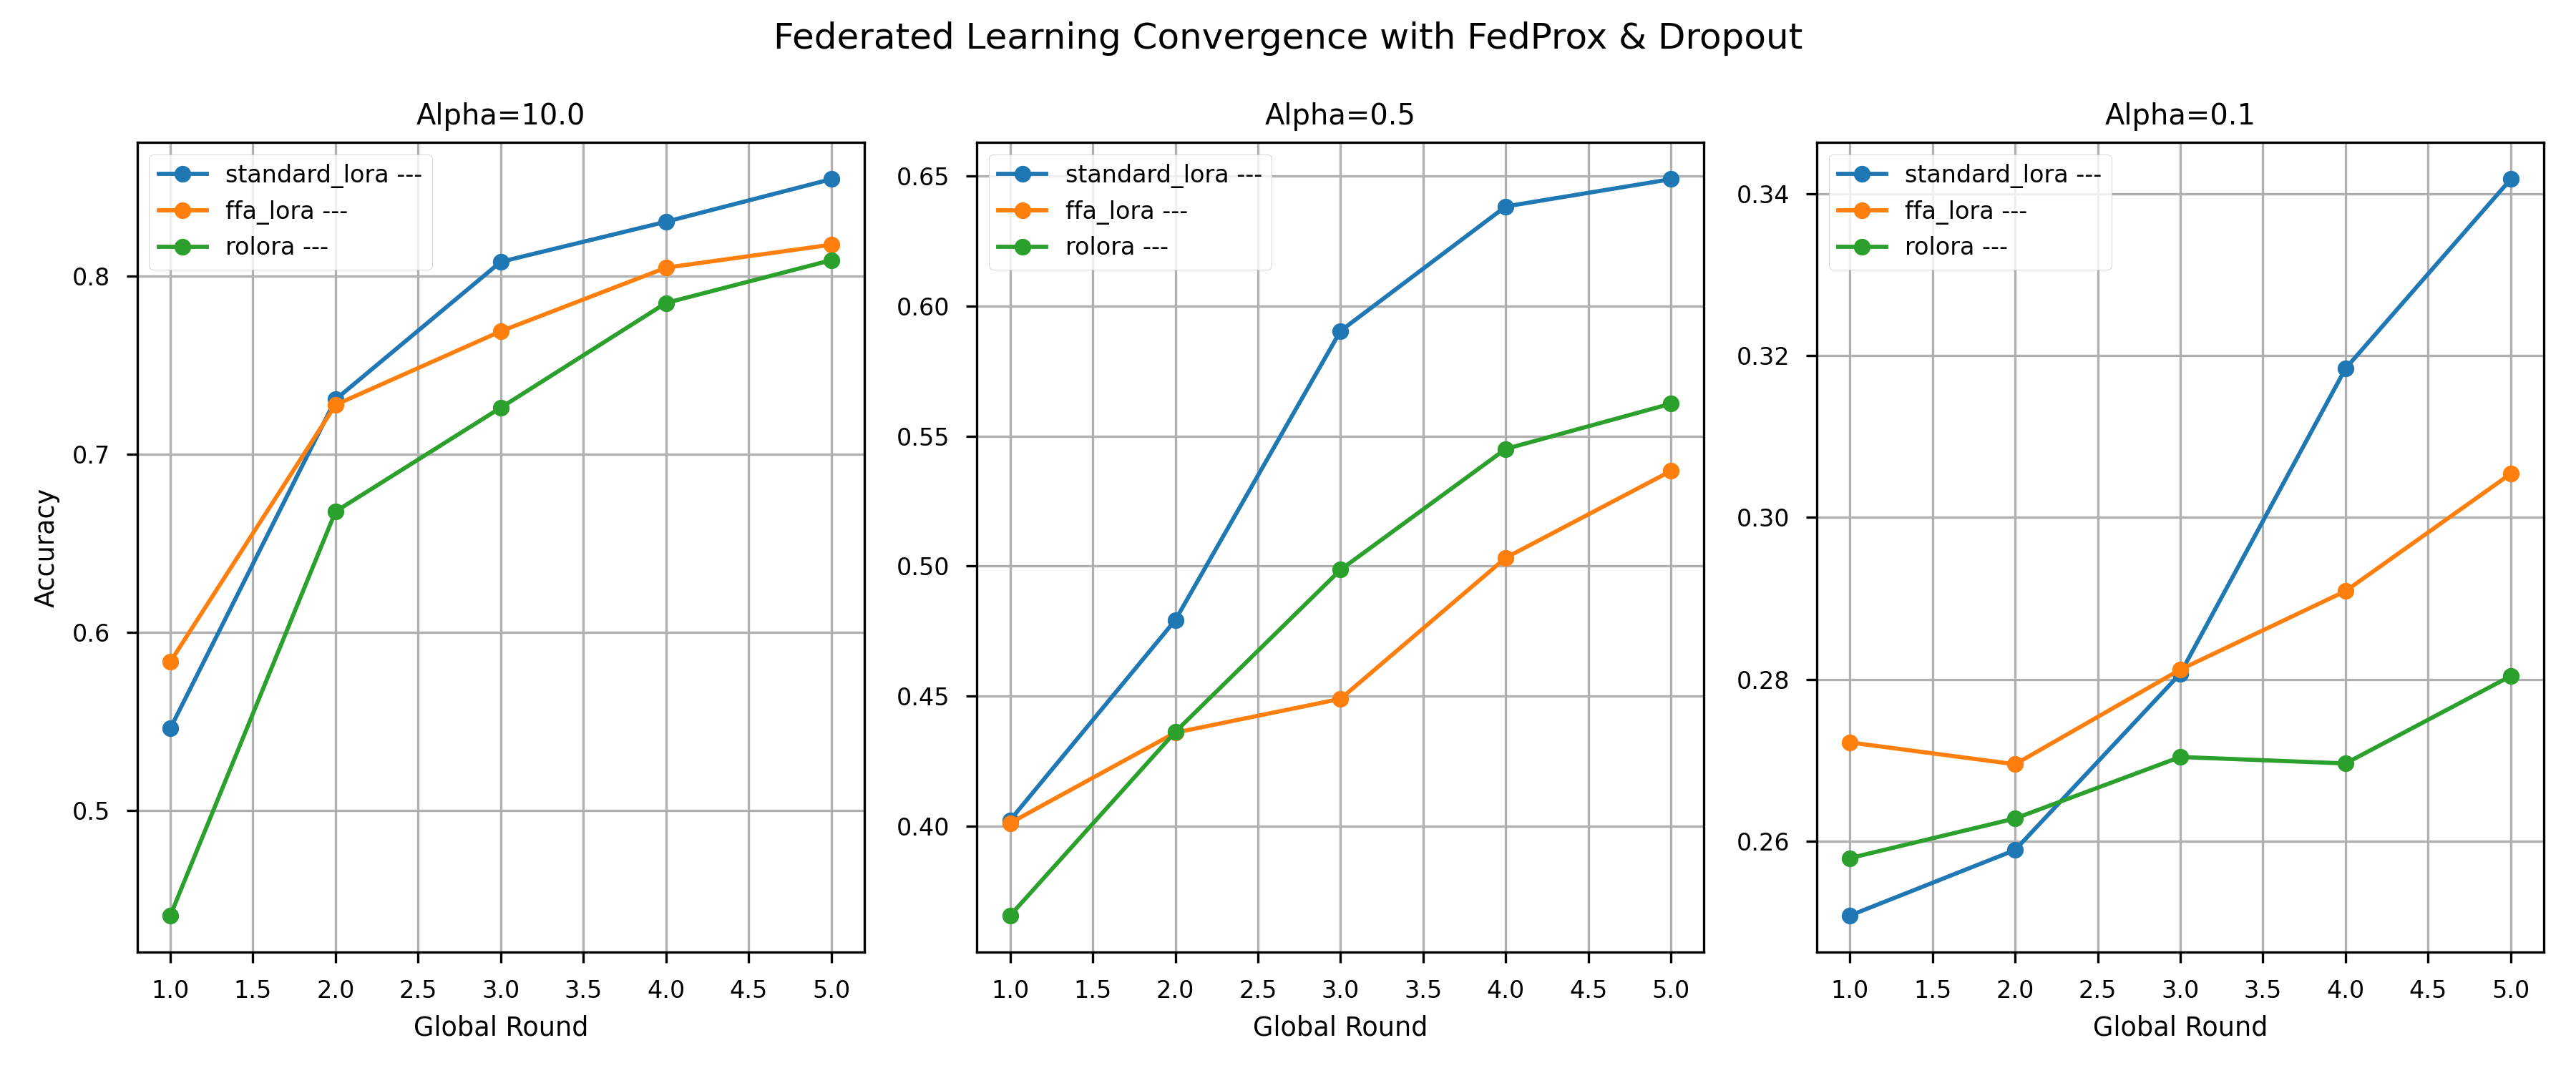
\includegraphics[width=\columnwidth]{../results/convergence_curves.png}
    \caption{Learning curves under simulated 20\% client dropout.}
    \label{fig:conv}
\end{figure}

\begin{figure}[h]
    \centering
    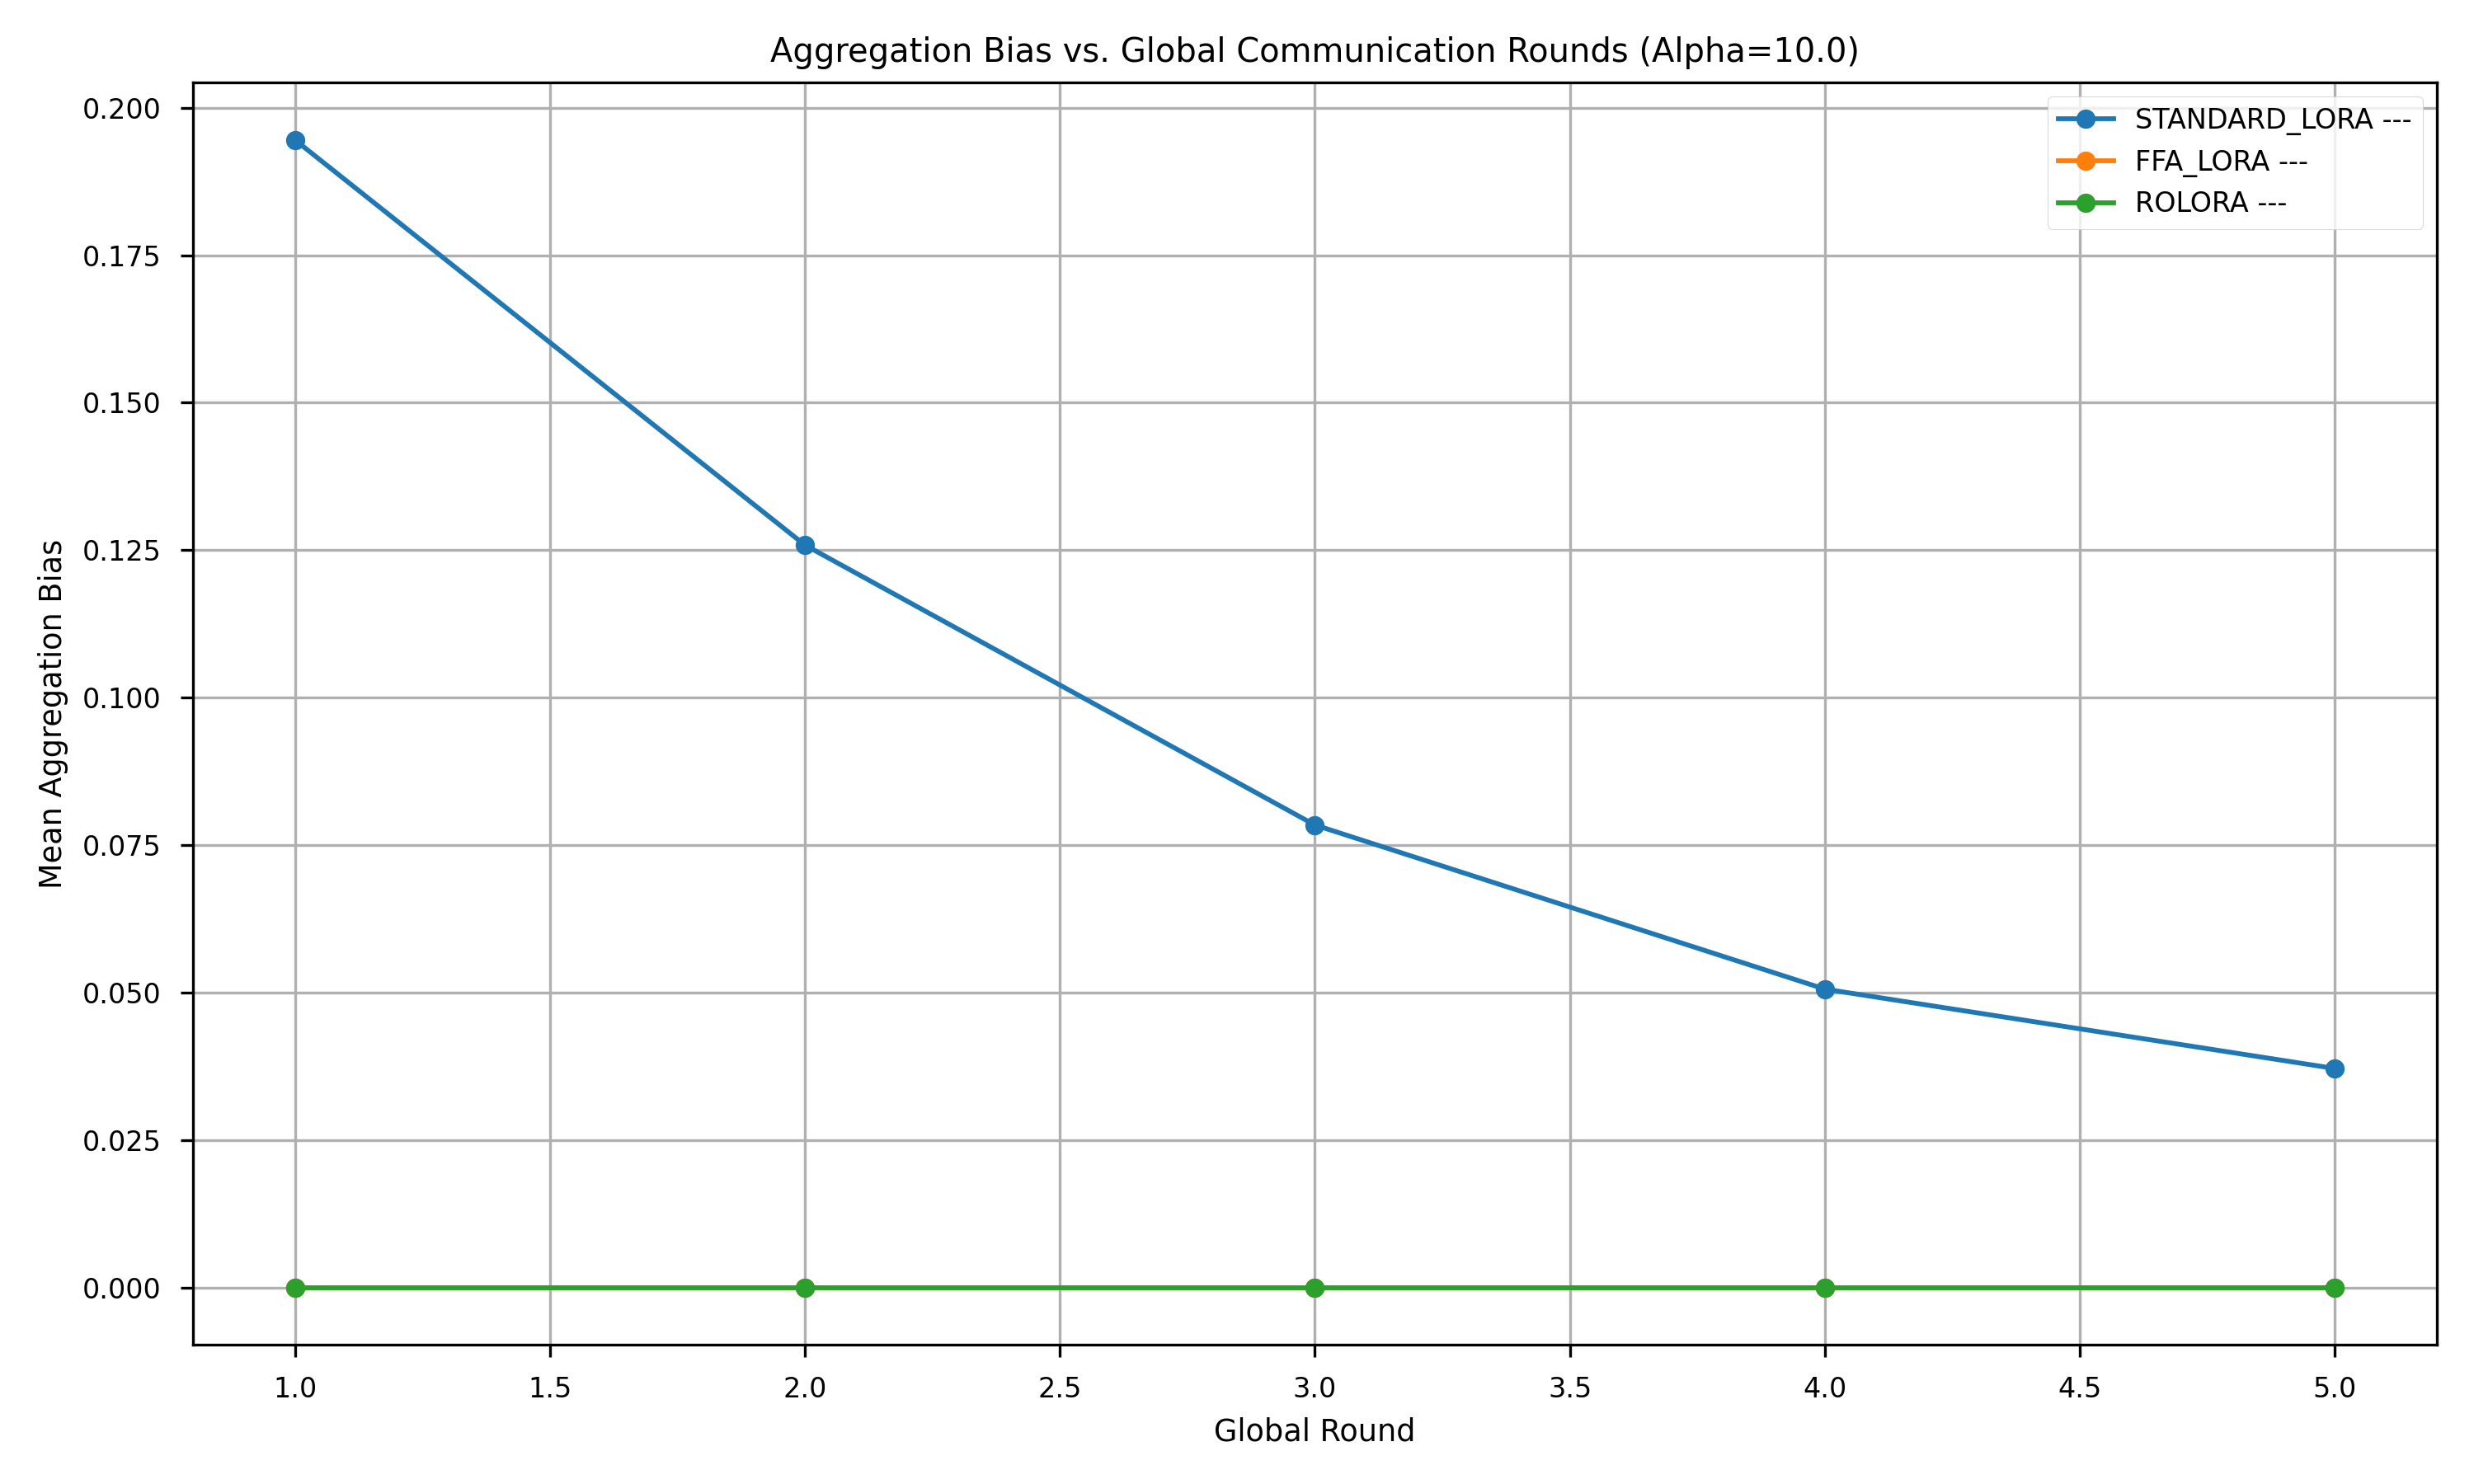
\includegraphics[width=\columnwidth]{../results/bias_curves.png}
    \caption{Mean Aggregation Bias vs. Global Communication Rounds.}
    \label{fig:bias}
\end{figure}

\section{Discussion: Scenarios, Advantages, and Trade-offs}
The choice of LoRA variant represents a strategic trade-off between capacity and efficiency. Standard LoRA is suitable for high-bandwidth environments where maximum expressivity is required. FFA-LoRA is ideal for ultra-low bandwidth scenarios, as it minimizes transmission to a single matrix and the classification head.

RoLoRA offers a balanced middle ground. While its alternating update mechanism reduces per-round bandwidth, our experiments exposed a vulnerability to asynchronous dropouts: if a client misses a round, its local $A$ and $B$ matrices may become temporally misaligned with the global state, leading to slightly lower performance compared to FFA-LoRA in extreme Non-IID settings. However, the successful implementation of heterogeneous rank aggregation via zero-padding demonstrates that FL can effectively incorporate diverse edge devices, allowing low-tier hardware ($r=4$) to contribute to a high-capacity global model ($r=8$) without introducing significant noise.

\section{Conclusion}
This study evaluated federated fine-tuning of LLMs under strict VRAM and bandwidth constraints. We demonstrated that RoLoRA and FFA-LoRA effectively eliminate aggregation bias and significantly reduce communication costs. While extreme data heterogeneity remains a challenge, the combination of FedProx and heterogeneous aggregation provides a robust foundation for real-world edge deployment.

\section{Future Work: Adaptive Rank Scheduling}
To further optimize the trade-offs explored in this paper, we propose a new algorithm: \textbf{Adaptive Bandwidth-Aware Rank Scheduling (ABARS)}. Unlike static rank allocation, ABARS dynamically adjusts the rank $r$ for each client based on real-time network throughput and VRAM availability. Furthermore, future research should explore \textit{Personalized Head Aggregation}, where the classification head is only partially averaged to mitigate the label-skew effects identified in our Non-IID analysis.

\appendices
\section{Experimental Mode Comparison}
The Quick Mode results obtained early in the study reached only 18.75\% accuracy for Standard LoRA ($\alpha=0.5$), compared to 64.89\% in Full Mode. This validates the necessity of sufficient training samples and communication rounds to achieve model convergence in federated LLM tasks.

\ifCLASSOPTIONcaptionsoff
  \newpage
\fi

\bibliographystyle{IEEEtran}
\bibliography{references}

\end{document}


